\lab{Conservation laws and heat flow}{Conservation laws and heat flow}
\label{lab:finitedifference1}

A conservation law is a balance law, and corresponds to an equation that describes how a quantity is balanced in some system throughout a given process.
(Consider how this is related to conservation laws in physics.)
For example, suppose we are keeping track of some measurable quantity in a physical system (e.g. heat, water, etc).
The fundamental conservation law then states that the rate of change of the total quantity in the system is equal to the rate of the quantity flowing into the system plus the rate at which the quantity is produced by sources inside the system.

\section*{Derivation of the Conservation equation in multiple dimensions}
Suppose $\Omega$ is a region in $\mathbb{R}^n$, and $V \subset \Omega$ is bounded with a reasonably well-behaved boundary $\partial V$.
Let $u(\vec{x},t)$ represent the density (concentration) of some quantity throughout $\Omega$.
Let $\vec{n}(x)$ represent the normal direction to $V$ at $x \in \partial V$, and let $\vec{J}(\vec{x},t)$ be the flux vector for the quantity, so that $\vec{J}(\vec{x},t) \cdot \vec{n}(x) \, dA$ represents the rate at which the quantity leaves $V$ by crossing a boundary element with area $dA$.
Note that the total amount of the quantity in $V$ is
\[ \int_V u(\vec{x},t)\, dt,\]
and the rate at which the quantity enters $V$ is
\[-\int_{\partial V} \vec{J}(\vec{x},t) \cdot \vec{n}(x) \, dA.\]

We let the source term be given by $f(\vec{x},t,u)$; we may interpret this to mean that the rate at which the quantity is produced in $V$ is
\[\int_V f(\vec{x},t,u)\, dt.\]
Then the integral form of the conservation law for $u$ is expressed as
\[\frac{d}{dt} \int_V u(\vec{x},t) \, d\vec{x} = -\int_V \vec{J}\cdot \vec{n}\, dA + \int_V f(\vec{x},t,u)\, d\vec{x}.\]

If $u$ and $J$ are sufficiently smooth functions, then we have
\[ \frac{d}{dt} \int_V u\, d\vec{x} = \int_V u_t \, d\vec{x},\]
and
\[ \int_V \vec{J}\cdot \vec{n}\, dA = \int_V \nabla \cdot \vec{J}\, d\vec{x} .\]
Since this holds for all nice subsets $V \subset \Omega$ with $V$ arbitrarily small, we obtain the differential form of the conservation law for $u$:
\[ u_t + \nabla \cdot \vec{J} = f(\vec{x},t,u) .\]

\section*{Constitutive Relations}
Currently our conservation law appears in the form
\[u_t + \nabla \vec{J} = f(\vec{x},t,u).\]
Thus the conservation law consists of one equation and 2 unknowns ($u$ and $J$).
To this equation we add other equations, called constitutive relations, which are used to fully determine the system.

For example, suppose we wish to describe the flow of heat.
Since heat flows from warmer regions to colder regions, and the rate of heat flow depends on the difference in temperature between regions, we usually assume that the flux vector $\vec{J}$ is given by
\[\vec{J}(x,t) = -\nu \nabla u(x,t),\]
where $\nu$ is a diffusion constant.
This constitutive relation is called Fick's law, and is the basic model for any diffusive process.
Substituting into the conservation law we obtain
\[u_t -\nu \triangle u(x,t) = f(\vec{x},t,u).\]
The function $f$ represents heat sources/sinks within the region.

\section*{Numerically modeling heat flow}
Consider the heat flow equation in one dimension together with appropriate initial conditions and homogeneous Dirichlet boundary conditions:
\begin{align*}
	&{ } u_t = \nu u_{xx}, \quad x \in [a,b],\quad t \in [0,T], \\
	&{ } u(a,t) = 0,\quad u(b,t) = 0,\\
	&{ } u(x,0) = f(x).
\end{align*}
We will look for an approximation $U^j_i$ to $u(x_i,t_j)$ on the grid $x_i = a +  hi$, $t_j = kj$, where $h$ and $k$ are small changes in $x$ and $t$ respectively and $i$ and $j$ are indices.
Note that the index $i$ ranges over different spacial grid points and the index $j$ ranges over different time steps.
We will denote the approximate value of $u$ at the $i$'th grid point and the $j$'th time step as $U_i^j$.

A common method for modeling ordinary and partial differential equations is the finite difference method, so-named because equations containing derivatives are replaced with equations containing difference schemes.
These difference schemes can often be found using Taylor's theorem.
For example, the equation
\begin{align*}
	u(x,t_j + k) = u(x,t_j) + u_t(x,t_j)k + \mathcal{O}(k^2)
\end{align*}
yields a first-order forward difference approximation to $u_t(x,t_j)$, namely,
\begin{align*}
	u_t(x,t_j ) = \frac{u(x,t_j+k) - u(x,t_j)}{k} + \mathcal{O}(k).
\end{align*}
Similarly, by adding the equations
\begin{align*}
	u(x_i+h,t) &= u(x_i,t) + u_x(x_i,t)h + u_{xx}(x_i,t)\frac{h^2}{2} + u_{xxx}(x_i,t)h^3 + \mathcal{O}(h^4),\\
	u(x_i-h,t) &= u(x_i,t) + u_x(x_i,t)(-h) + u_{xx}(x_i,t)\frac{(-h)^2}{2} + u_{xxx}(x_i,t)(-h)^3 + \mathcal{O}(h^4),
\end{align*}
we obtain a second-order centered difference approximation to $u_{xx}(x_i,t)$:
\begin{align*}
	u_{xx}(x_i,t_j) &= \frac{u(x_i + h,t_j )-2 u(x_i,t_j)- u(x_i - h,t_j)}{h^2} + \mathcal{O}(h^2).
\end{align*}

\begin{figure}
\centering
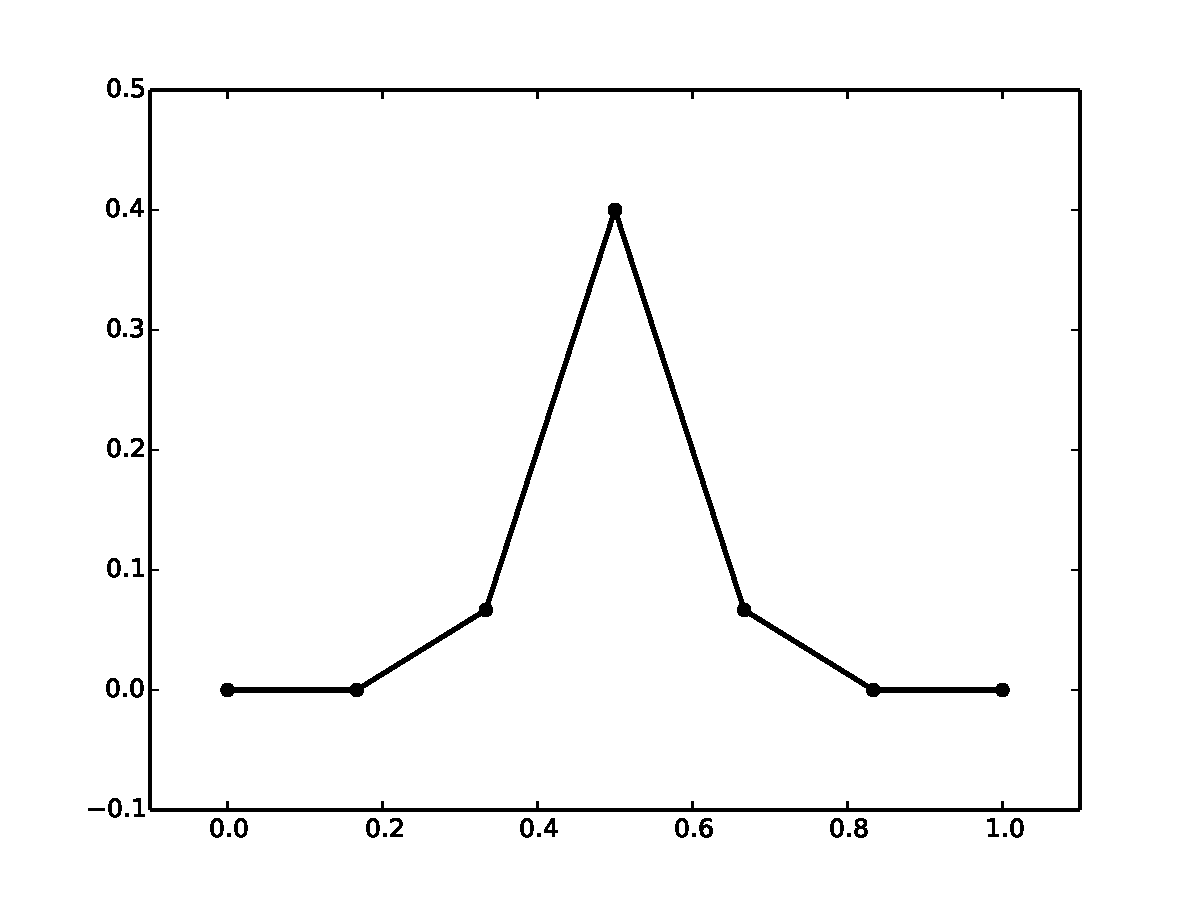
\includegraphics[width=\textwidth]{heatexercise1a.pdf}
\caption{The graph of $U^{0}$, the approximation to the solution $u(x,t=0)$ for Problem \ref{prob:heat_exercise1}.}
\label{fig:heatexercise1a}
\end{figure}

% A simple explicit method for numerically approximating the solution of this problem is to use a forward difference approximation in time and a centered difference approximation in space.
% Recall that
% \[u_t(x_i,t_j) = \frac{u(x_i,t_j + k) - u(x_i,t_j)}{k} + \mathcal{O}(k)
% \]
%  and
% \[u_{xx}(x_i,t_j) = \frac{u(x_i + h,t_j )-2 u(x_i,t_j)- u(x_i - h,t_j)}{h^2} + \mathcal{O}(h^2).
% \]
% Let $U_{i,j}$ represent our approximation to $u(x_i,t_j)$.
These difference approximations give us the $\mathcal{O}(h^2 + k)$ explicit method
\begin{align}
	\begin{split}
	\frac{U_{i}^{j+1} - U_{i}^{j}}{k} &= \nu \frac{U_{i+1}^{j}- 2U_{i}^{j} + U_{i-1}^{j} }{h^2} ,\\
	U_{i}^{j+1} &= U_{i}^{j} + \frac{\nu k}{h^2} (U_{i+1}^{j}- 2U_{i}^{j} + U_{i-1}^{j} ).
	\end{split}\label{eqn:firstorder_explicit}
\end{align}
This method can be written in matrix form as
\[U^{j+1} = A U^j,\]
where $A$ is the tridiagonal matrix given by
\[A = \left[\begin{array}{cccccc}1-2\lambda & \lambda & & & \\ \lambda & 1-2\lambda & \lambda & & \\ & \ddots & \ddots & \ddots & \\ & & \lambda & 1-2\lambda & \lambda \\  &  &  & \lambda & 1-2\lambda\end{array}\right],\]
$\lambda = \nu k/h^2$, and $U^j$ represents the approximation at time $t_j$.
We can get this method started by using the initial condition given in our problem, so that $U_{i}^{0} = f(x_i)$.

\begin{figure}
\centering
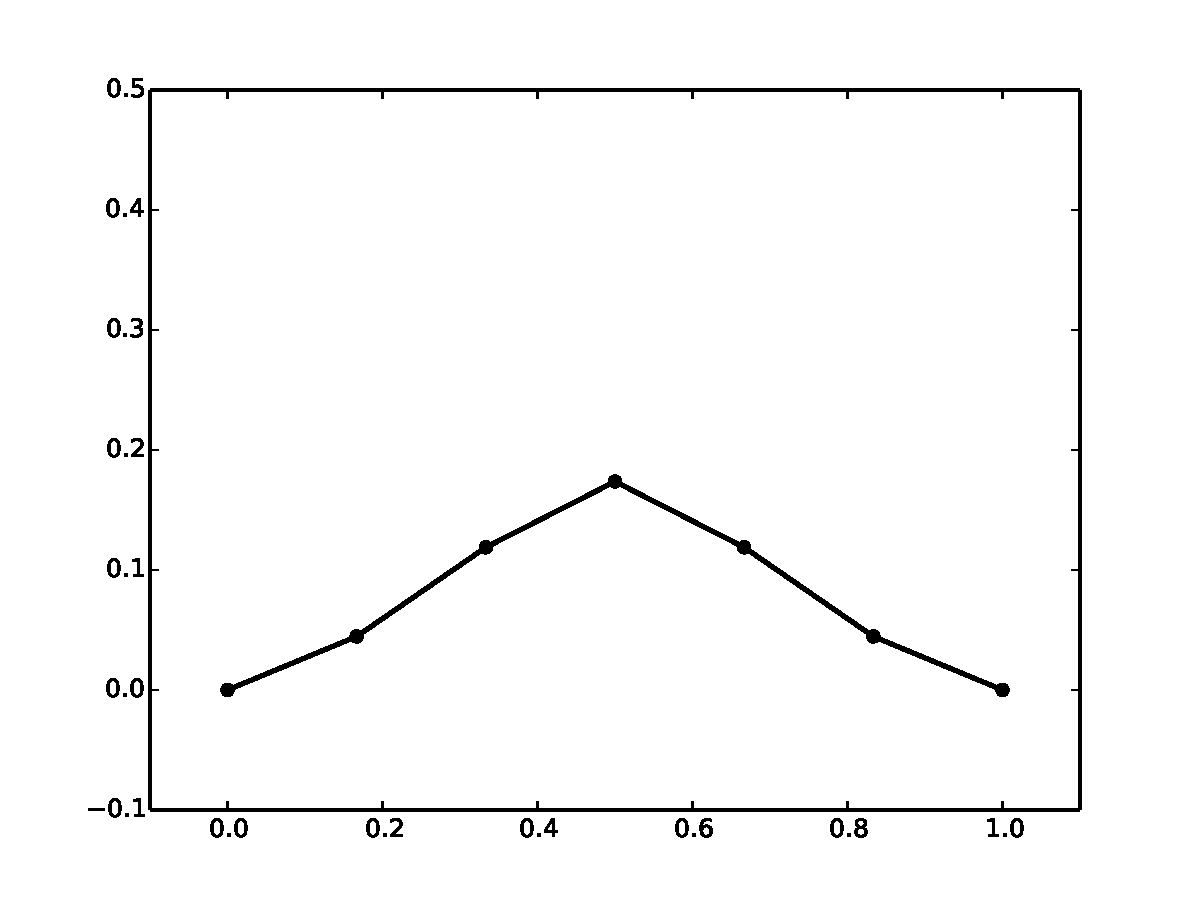
\includegraphics[width=\textwidth]{heatexercise1b.pdf}
\caption{The graph of $U^{10}$, the approximation to the solution $u(x,t=.4)$ for Problem \ref{prob:heat_exercise1}.}
\label{fig:heatexercise1b}
\end{figure}

\begin{info}
Finite difference schemes, though they can be \emph{represented} using matrix multiplication, should not be \emph{implemented} using raw matrix multiplication.
Using NumPy, it is best to vectorize the difference scheme so that you do not have to loop over the spatial indices.
If you are using a language with faster loops (like C, C++, Fortran, or Cython), it could work well to loop directly through the indices in both time and space.
\end{info}

To account for boundary conditions using this differencing scheme, simply set the boundary points to the appropriate values in the initial conditions, then avoid modifying them as you update for each time step.
This would be the equivalent of replacing the first and last rows of the matrix representation of the differencing scheme with the first and last rows of the identity matrix.

\begin{problem}
\label{prob:heat_exercise1}
Consider the specific initial boundary value problem
\begin{align}
	\begin{split}
	&{ } u_t = .05 u_{xx}, \quad x \in [0,1], \\
	&{ } u(0,t) = 0,\quad u(1,t) = 0,\\
	&{ } u(x,0) = 2\max\{.2 - |x-.5|,0\}.
	\end{split}
\end{align}
Approximate the solution $u(x,t)$ at time $t = .4$ be taking 6 subintervals in the $x$ dimension and 10 subintervals in time.
The graphs for $U^0$ and $U^{10}$ are given in Figures \ref{fig:heatexercise1a} and \ref{fig:heatexercise1b}.
\end{problem}

For the next problem, we need to show how Matplotlib can be used to create a 2D animation.
The following is a simple working example that animates a sine wave.

% Note: If an animation is running slowly, consider using the \li{blit=True} option when creating the animation.
% If you do this, also define an initialization function that sets the line's data to empty lists and returns a 1-tuple containing the line object.
% Pass the initialization function to the \li{FuncAnimation} function using the \li{init_func} keyword argument.

\begin{lstlisting}
import numpy as np
from matplotlib import animation, pyplot as plt

def sine_animation(res=100):
    # Make the x and y data.
    x = np.linspace(-1, 1, res+1)[:-1]
    y = np.sin(np.pi * x)
    # Initialize a matplotlib figure.
    f = plt.figure()
    # Set the x and y axes by constructing an axes object.
    plt.axes(xlim=(-1,1), ylim=(-1,1))
    # Plot an empty line to use in the animation.
    # Notice that we are unpacking a tuple of length 1.
    line, = plt.plot([], [])
    # Define an animation function that will update the line to
    # reflect the desired data for the i'th frame.
    def animate(i):
        # Set the data for updated version of the line.
        line.set_data(x, np.roll(y, i))
        # Notice that this returns a tuple of length 1.
        return line,
    # Create the animation object.
    # 'frames' is the number of frames before the animation should repeat.
    # 'interval' is the amount of time to wait before updating the plot.
    # Be sure to assign the animation a name so that Python does not
    # immediately garbage collect (delete) the object.
    a = animation.FuncAnimation(f, animate, frames=y.size, interval=20)
    # Show the animation.
    plt.show()

# Run the animation function we just defined.
sine_animation()
\end{lstlisting}

\begin{problem}
\label{prob:heat_exercise2}
Solve the specific initial boundary value problem
\begin{align}
	\begin{split}
	&{ } u_t = u_{xx}, \quad x \in [-12,12],\quad t \in [0,1], \\
	&{ } u(-12,t) = 0,\quad u(12,t) = 0,\\
	&{ } u(x,0) = \max\{1 - x^2,0\}
	\end{split}
\end{align}
using the first order explicit method \ref{eqn:firstorder_explicit}.
Use 140 subintervals in the $x$ dimension and 70 subintervals in time.
The initial and final states are shown in Figure \ref{fig:heatexercise2}.
Animate your results.

Explicit methods usually have a stability condition, called a CFL condition (for Courant-Friedrichs-Lewy).
For method \ref{eqn:firstorder_explicit} the CFL condition that must be satisfied is that
\[\lambda \leq \frac{1}{2}.\]
Repeat your computations using 140 subintervals in the $x$ dimension and 66 subintervals in time.
For these values the CFL condition is broken; you should easily see the result of this instability in the approximation $U^{66}$.
% Then the graphs for $U^0$ and $U^{70}$ are given in \eqref{heatexercise2a} and \ref{heatexercise2b}.
\end{problem}

\begin{figure}
\centering
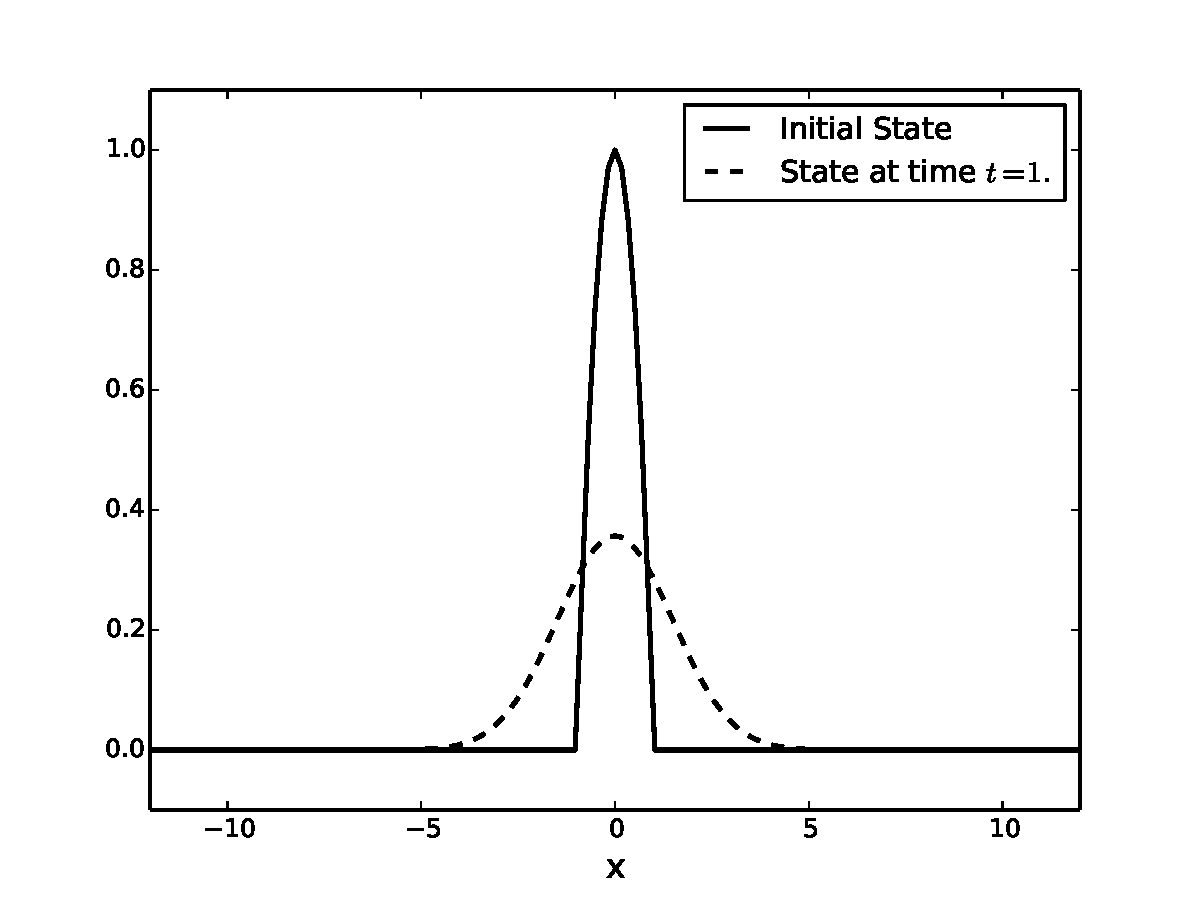
\includegraphics[width=\textwidth]{heatexercise2.pdf}
\caption{The initial and final states for equation Problem \ref{prob:heat_exercise2}.}
\label{fig:heatexercise2}
\end{figure}

Implicit methods often have better stability properties than explicit methods.
The Crank-Nicolson method, for example, is unconditionally stable and has order $\mathcal{O}(h^2 + k^2)$.
To derive the Crank-Nicolson method, we use the following approximations:
\begin{align*}
	u_t(x_i,t_{j+1/2}) &= \frac{u_t(x_i,t_{j+1}) - u_t(x_i,t_j)}{k} + \mathcal{O}(k^2), \\
	u_{xx}(x_i,t_{j+1/2}) &= \frac{u_{xx}(x_i,t_{j+1}) + u_{xx}(x_i,t_j)}{2} + \mathcal{O}(k^2).
\end{align*}
These approximations give the method
\begin{align}
	\begin{split}
	\frac{U^{j+1}_i - U^j_i}{k} &= \frac{1}{2}\left( \frac{U^j_{i+1} - 2U^j_{i} + U^j_{i-1}}{h^2} + \frac{U^{j+1}_{i+1} - 2U^{j+1}_{i} + U^{j+1}_{i-1}}{h^2}  \right) ,\\
	U^{j+1}_i  &= U^j_i + \frac{k}{2h^2} \left( U^j_{i+1} - 2U^j_{i} + U^j_{i-1} + U^{j+1}_{i+1} - 2U^{j+1}_{i} + U^{j+1}_{i-1}   \right).
\end{split}
\end{align}
This method can be written in matrix form as
\[BU^{j+1} = A U^j,\]
where $A$ and $B$ are tridiagonal matrices given by
\begin{align*}
B &= \left[\begin{array}{cccccc}1+2\lambda & -\lambda &  &  &  \\ -\lambda & 1+2\lambda &  -\lambda & &  \\ &  \ddots &   \ddots & \ddots \\ & &  -\lambda &  1+2\lambda & -\lambda \\ &  &  & -\lambda & 1+2\lambda\end{array}\right], \\
A &= \left[\begin{array}{cccccc}1-2\lambda & \lambda &  &  &  \\ \lambda & 1-2\lambda &  \lambda & &  \\ &  \ddots &   \ddots & \ddots \\ & &  \lambda &  1-2\lambda & \lambda \\ &  &  & \lambda & 1-2\lambda\end{array}\right],
\end{align*}
where $\lambda = \nu k/(2h^2)$, and $U^j$ represents the approximation at time $t_j$.
Note that here we have defined $\lambda$ differently than we did before!

How do we know if a numerical approximation is reasonable?
One way to determine this is to compute solutions for various step sizes $h$ and see if the solutions are converging to something.
To be more specific, suppose our finite difference method is $\mathcal{O}(h^p)$ accurate.
This means that the error $E(h) \approx Ch^p$ for some constant $C$ as $h \to 0$ (i.e., for $h>0$ small enough).

So compute the approximation $y_k$ for each stepsize $h_k$, $h_1 > h_2> \ldots>h_m.$
We will think of $y_m$ as the true solution.
Then the error of the approximation for stepsize $h_k, k < m,$ is
\begin{align*}
	E(h_k) &= \max( \abs{ y_k - y_m}) \approx C h_k^p ,\\
	\log(E(h_k)) &= \log(C) + p \log(h_k).
\end{align*}
Thus on a log-log plot of $E(h)$ vs. $h,$ these values should be on a straight line with slope $p$ when $h$ is small enough to start getting convergence.

\begin{figure}
\centering
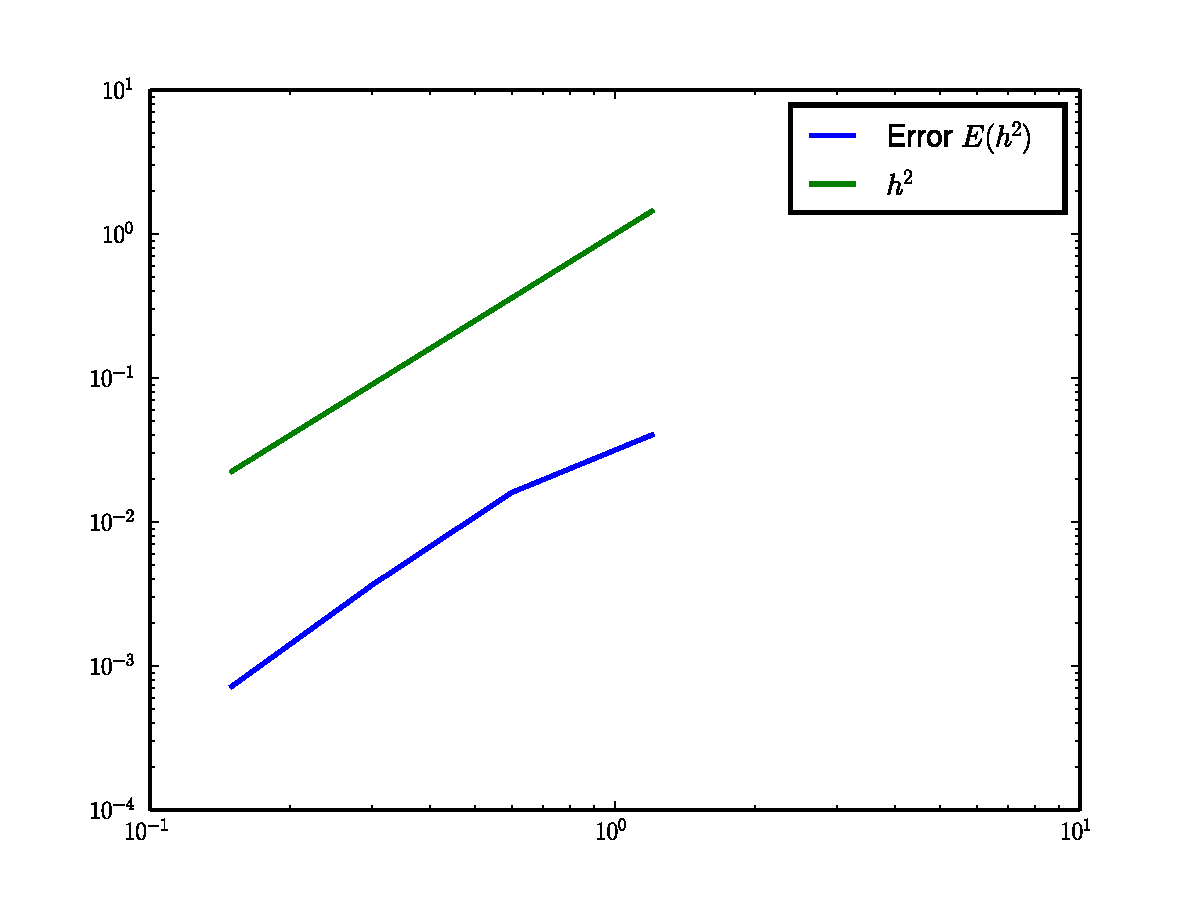
\includegraphics[width=\textwidth]{MaximumError.pdf}
\caption{$E(h)$ represents the (approximate) maximum error in the numerical solution $U$ to Problem \ref{prob:heat_exercise3} at time $t=1$, using a stepsize of $h$.}
\label{fig:heatexercise3}
\end{figure}

% If dgtsv is ever included in SciPy, it would probably be better to use that here instead of a custom routine.
When implementing the Crank-Nicolson method, you will need some way to solve a tridiagonal system.
The following is a simple function that performs a tridiagonal solve.
\li{a}, \li{b}, and \li{c} are assumed to contain the first subdiagonal, main diagonal, and first superdiagonal of the tridiagonal matrix.
\li{x} is assumed to be the right hand side of the equation.
This function overwrites \li{x} with the solution to the system.
As has been shown in earlier labs, this function is better implemented in Cython, C, Fortran, or some other language with less overhead for array accesses and loops.
\begin{lstlisting}
def tridiag(a, b, c, x):
    # Overrides c and x.
    # The contents of x after computation will be the solution to the system.
    size = x.size
    temp = 0.
    c[0] = c[0] / b[0]
    x[0] = x[0] / b[0]
    for n in range(size-2):
        temp = 1. / (b[n+1] - a[n]*c[n])
        c[n+1] *= temp
        x[n+1] = (x[n+1] - a[n]*x[n]) * temp
    x[size-1] = (x[size-1] - a[size-2]*x[size-2]) / (b[size-1] - a[size-2]*c[size-2])
    for n in range(b.size-2, -1, -1):
        x[n] = x[n] - c[n] * x[n+1]
\end{lstlisting}

To account for boundary conditions when using the Crank-Nicolson method, set the boundary points at the beginning of the iteration and leave them constant when applying $A$ like you did before.
In the Tridiagonal solve, replace the first row of the matrix $B$ with the first row of the identity and the last row of the matrix $B$ with the last row of the identity.

\begin{problem}
\label{prob:heat_exercise3}
Using the Crank Nicolson method, numerically approximate the solution $u(x,t)$ of the problem
\begin{align}
	\begin{split}
	&{ } u_t = u_{xx}, \quad x \in [-12,12],\quad t \in [0,1],\\
	&{ } u(0,t) = 0,\quad u(1,t) = 0,\\
	&{ } u(x,0) = \max\{1 - x^2,0\}.
	\end{split}
\end{align}
Demonstrate that the numerical approximation at $t = 1$ converges to  $u(x,t=1)$.
Do this by computing $U$ at $t=1$ using $20,40,80,160,320$, and $640$ steps.
Use the same number of steps in both time and space.
Reproduce the loglog plot shown in Figure \ref{fig:heatexercise3}.
The slope of the line there shows the proper rate of convergence.

To measure the error, use the solution with the smallest $h$ (largest number of intervals) as if it were the exact solution, then sample each solution only at the x-values that are represented in the solution with the largest $h$ (smallest number of intervals).
Use the $\infty$-norm on the arrays of values at those points to measure the error.

Notice that, since the Crank-Nicolson method is unconditionally stable, there is no CFL condition and we can use the same number of spaces in time and space.
\end{problem}

% The matrix $A$ is sparse, and so we can use several functions from the package \texttt{scipy.sparse.linalg}.
% In particular, we use the functions \texttt{spdiags} and \texttt{spsolve}.
%
% \begin{verbatim}
% D1,D2,D3 = -4*np.ones((1,m**2)), np.ones((1,m**2)), np.ones((1,m**2))
% Dm = np.ones((1,m**2))
% for j in range(0,D2.shape[1]):
%     if (j%m)==m-1:
%         D2[0,j]=0
%         if (j%m)==0:
%             D3[0,j]=a0
% diags = np.array([0,-1,1,-m,m])
% data = np.concatenate((D1,D2,D3,Dm,Dm),axis=0)
%
% A = 1./h**2.*spdiags(data, diags, m**2,m**2).asformat('csr')
% \end{verbatim}
%
% \subsection{2D Heat Equation}
% Recall that the collection of finite difference equations
% \[
% \nabla^2_h U_{ij} = 0, \quad 1 \leq i,j\leq m,
% \]
% can be written in matrix form as
% $$AU + q  = 0$$
%
% The Crank-Nicolson method for the 2D heat equation is given by
% \[U_{i,\,j}^{n+1}- U_{i,\,j}^{n} = \frac{\Delta t}{2}(\nabla_h^2 U_{i,\,j}^{n} + \nabla_h^2 U_{i,\,j}^{n+1}) \text{ for each } 1 \leq i,j \leq m, \]
% is a second order accurate in both space and time. Basically we're using a midpoint scheme in time,
% and a trapezoidal scheme in space. The resulting method is implicit, and can be written in matrix form as
% \begin{align*}
% 	IU^{n+1} &= IU^n + \frac{\Delta t}{2}(AU^n + q + AU^{n+1} + q),\\
% 	(I - \frac{\Delta t}{2}A)U^{n+1}&= (I + \frac{\Delta t}{2}A)U^n + \Delta t q.	
% \end{align*}
%
% TODO: What size must the time step be to ensure stability?
%
% We will need to take many time steps, where many equations must be solved with the matrix $(I - \frac{\Delta t}{2}A)$.
% The function \texttt{factorized} from \texttt{scipy.sparse.linalg} computes the LU decomposition of the matrix.
% This decomposition reduces the time required for solving consecutive time steps.
% 